\documentclass{article}
\usepackage[T1]{fontenc}
\usepackage{geometry}
\geometry{
	a4paper,
	total={170mm,257mm},
	left=20mm,
	top=20mm,
}
\usepackage{graphicx}
\usepackage{titling}
\usepackage[most]{tcolorbox}

\title{Feasibility of Machine Learning Applied to the Field of Ant Venom Peptides}
\author{Hao ZHANG}
\date{September 8, 2023 }

\usepackage{fancyhdr}
\pagestyle{fancy}
\fancypagestyle{plain}{
	\fancyhf{}
	\fancyhead[L]{\thetitle}
	\fancyhead[R]{\theauthor}
	\fancyfoot[L]{\thedate}
	\fancyfoot[C]{\vskip -10pt
\includegraphics[width=1cm]{My_Seal.png}}
	\fancyfoot[R]{\thepage}
}
\fancyhf{}
\fancyhead[L]{\thetitle}
\fancyhead[R]{\theauthor}
\fancyfoot[L]{\thedate}
\fancyfoot[C]{\vskip -10pt
\includegraphics[width=1cm]{My_Seal.png}}
\fancyfoot[R]{\thepage}
\makeatletter
\def\@maketitle{
	\newpage
	\null
	\vskip 1em
	\begin{center}
		\let \footnote \thanks
		{\LARGE \@title \par}
		\vskip 1em
	\end{center}
	\par
	\vskip 1em}
\makeatother

\usepackage{lipsum}  
\usepackage{cmbright}

\makeatletter
\renewcommand\paragraph{\@startsection{paragraph}{4}{\z@}%
	{3.25ex \@plus1ex \@minus.2ex}%
	{-1em}%
	{\normalfont\normalsize}}
\makeatother

\begin{document}
	
	\maketitle
	
	%\hrule
	%\vskip 2em
	%\noindent\begin{tabular}{@{}ll}
		%	Article Title & An Overview of Artificial Intelligence in Product Design for Smart Manufacturing\\
		%	Article Authors & Janjira Aphirakmethawong, Erfu Yang, and Jörn Mehnen\\
		%	Publication Information &  Proceedings of the 27th International Conference on Automation \& Computing, \\ & University of the West of England, Bristol, UK, 1-3 September 2022
		%\end{tabular}
		%\vskip 2em
		%\noindent\dotfill
		
		\section*{Studies Related to Ant Venom Peptides}
		
		\paragraph*{Venoms are complex biochemical mixtures consisting of a large number of biologically active compounds. Venoms exhibit remarkable biochemical complexity, ranging from small molecules to large proteins, fine-tuned by nature for greater efficacy and target selectivity. Peptides are the main components of most arthropod venoms and are being investigated for their potential as therapeutic lead compounds, molecular probes or insect-selective biopesticides.}
		
		\paragraph*{Ants (Hymenoptera: Formicidae) are a diverse but also neglected group of venomous arthropods. Extremely diverse and ubiquitous in terrestrial environments, ants can be considered one of the most abundant groups of venomous animals on Earth. Compared to other animal venoms, ant venoms have been little studied. Ants have evolved complex venoms that rapidly immobilize arthropod prey and protect their colonies from predators and pathogens. Many ants retain peptide-rich venoms that are similar to those of other arthropods. It has been shown that the peptide composition of venoms produced by a variety of ants is as complex as that of spiders, scorpions or cone snails, and it has been estimated that ant venoms contain an average of 130 unique peptides\textsuperscript{\cite{ref1}} . With the development of micro-bioassay techniques and the increased sensitivity of mass spectrometry and nuclear magnetic resonance spectroscopy, it is now possible to study more extensively the small amounts of venom peptides provided by small animals, especially ants, and recent advances in mass spectrometry, in particular, have begun to reveal the true complexity of the composition of ant venom peptides\textsuperscript{\cite{ref2}} .}
		
		\paragraph*{The 2018 BTSB-EA7417 team used a direct transcriptomics approach (RT-PCR-based cloning) to confirm and complete cDNA sequences and gene expression in the venom glands and identified a total of 37 peptide toxin precursors, which further clustering analyses were able to categorize into three superfamilies, which are processed into thousands of peptides in the venom\textsuperscript{\cite{ref3}}. The team has now identified about 100 potentially bioactive peptides from ant venom. Some of them disrupt cell membranes, while others are not cytotoxic and their mechanisms of action are more specific and still unknown. Therefore, the full identification and understanding of their targets and their actions are decisive for their future commercial use.}
		
		\section*{Planarians in Toxicology Research}
		
		\paragraph*{In toxicology research, there is a need to follow the guidelines for the human use of animals in scientific research, also known as the three Rs (replace, reduce, and refine). Invertebrates are useful experimental organisms for the study of biological and toxicological problems due to their unique biological characteristics such as relatively simple body structures and systems, short life cycles and diverse reproductive strategies. The application of invertebrate species to ecological and environmental toxicology not only typically reduces the cost of maintenance and the difficulty of experimental manipulation, but also generates useful toxicological information from the individual to the population or community level.}
		
		\paragraph*{Planarians are distributed throughout the world and are readily available for scientific purposes. Planarians are invertebrates that have received a great deal of attention from scientists over the past three decades, and the place of planarians in biological research has been widely recognized by scientists in a variety of fields. The use of planarians in toxicological studies seems promising. Planarians are often used to examine the toxicity of exogenous chemicals, especially those produced by human activities. The results of many toxicological studies to date collectively suggest that planarians are ideal test organisms for examining toxicity. planarians have been used to study genotoxicity, tumorigenicity, neurotoxicity, and reproductive toxicity; this suggests that they are potentially powerful tools in the field of ecological and environmental toxicology for comprehensively examining the effects of chemicals and providing critical information generated by risk assessment\textsuperscript{\cite{ref4}}.}
		
		\section*{Challenges of Machine Learning in Biological Applications}
		
		\paragraph*{The term "machine learning" broadly refers to the process of fitting data with predictive models or identifying groups of information in data. Machine learning is useful when one wants to analyze a dataset that is too large (many individual data points) or too complex (contains a large number of features) to analyze manually, or when one needs to automate the process of analyzing the data in order to create repeatable and time-saving workflows. This is often the case with data from biological experiments. The size and complexity of biological datasets have grown dramatically over the past few decades. As a result, it has become increasingly important to have a thorough understanding of these techniques used, in addition to some practical methods that can be used to interpret large amounts of data. Machine learning has been used in biology for decades, but it has steadily grown in importance and has been applied to almost every area of biology. However, it is only in the last few years that the field has begun to take a more critical look at the available strategies and has begun to evaluate which methods are most appropriate, or not at all, in different scenarios\textsuperscript{\cite{ref5}}.}
		
		\paragraph*{Current challenges to machine learning in biological applications include issues of data availability (huge amounts of data in some areas and very small amounts in others), data leakage, and interpretability of models. Therefore there is a need to focus on privacy-preserving machine learning that allows data sharing and distributed training of machine learning models in the context of data privacy, and algorithms have been developed for efficient federated model training using data stored in different locations. Also interdisciplinary collaboration is necessary; rarely is a research group able to both collect data for machine learning research and efficiently apply the most appropriate machine learning methods unless publicly available data are used. It is common for experimental biologists to collaborate with computer scientists, and such collaborations usually yield good results. However, in such collaborations, it is important that both parties have some working knowledge of the other. In particular, the computer scientist should endeavor to understand the data, e.g., the expected level of noise and reproducibility, and the biologist should understand the limitations of the machine-learning algorithms used. Building such understanding takes time and effort, but is important to prevent unintentional propagation of bad models and misleading results.}
		
		\section*{Selection of Machine Learning Methods}
		
		\paragraph*{There are two goals for using machine learning in biology. The first is to make accurate predictions where there is a lack of experimental data and to use these predictions to guide future research. The second goal is to use machine learning to further our understanding of biology. However, these two goals often conflict. Due to the variety of data types encountered in the field of biology, choosing the right machine learning or rather deep learning method based on the problem to be solved and the type of data available becomes crucial to obtaining effective results. Figure 1 provides a decision tree for the entire process of training a machine learning method to help researchers select a model\textsuperscript{\cite{ref5}}. The flowchart is intended as a visual guide to connect the concepts outlined in this review. Of course, such a simple overview does not cover all situations, and it is still necessary to select the appropriate machine learning method based on the specific data content and the goals of the task.}
		
		\begin{figure}[hbtp]
			\centering 
			\fboxrule = 1.2pt 
			\fboxsep = 0pt 
			\fcolorbox{white}{white}{
				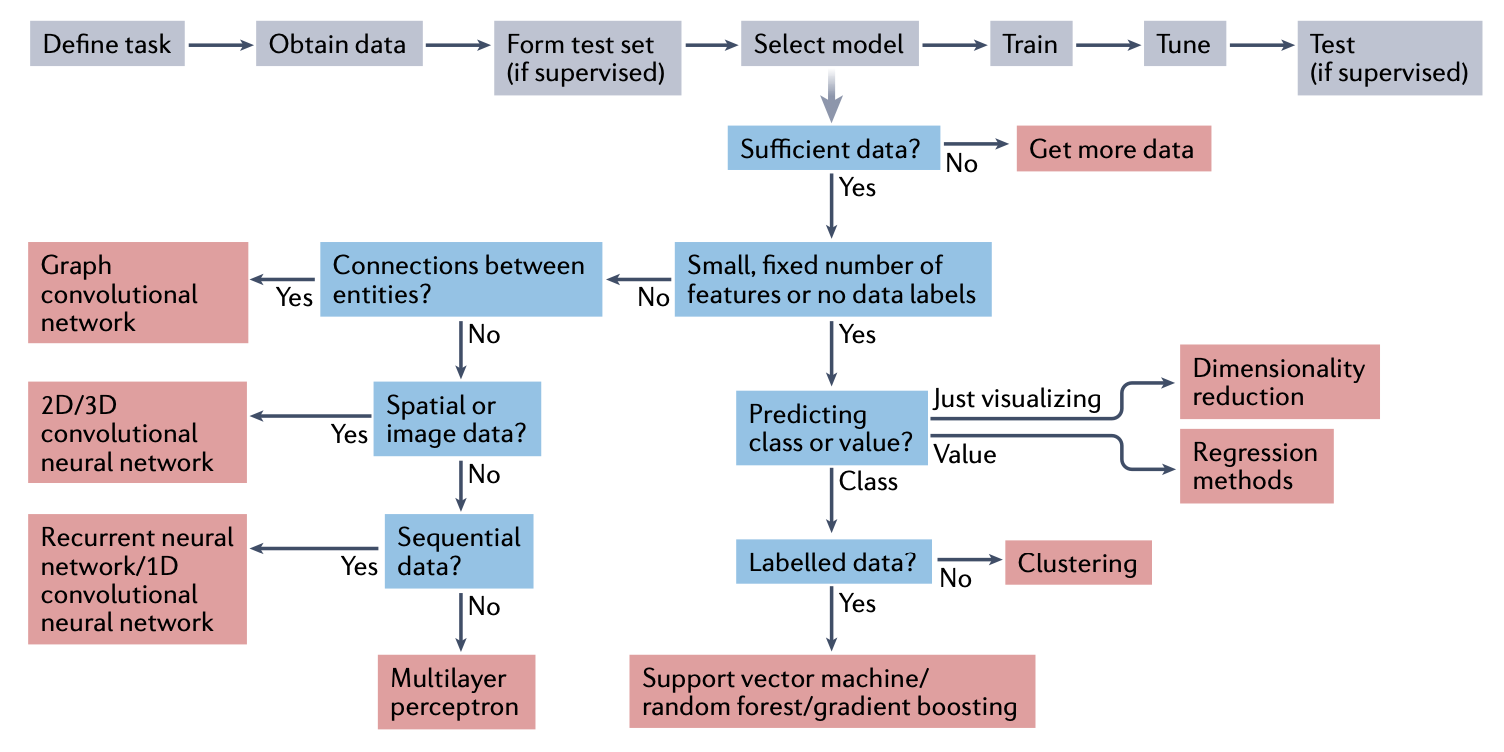
\includegraphics[width = 1\linewidth]{figures/figure_1.png}}
			\caption{Choosing and training a machine learning method}	
		\end{figure}
		
		\paragraph*{Perhaps the biggest challenge to modeling biological data is the sheer variety. The data that biologists need to work with include gene and protein sequences, gene expression levels over time, evolutionary trees, microscope images, 3D structures and interaction networks, and more. Some best practices and important considerations for specific biological data types are summarized in Figure 2\textsuperscript{\cite{ref5}}. Due to the variety of data types encountered, biological data often requires customized solutions to be processed effectively, making it difficult to recommend off-the-shelf tools or even general guidelines for using machine learning in these problem domains, as the choice of models, training process, and test data depends heavily on the specific question one wants to answer. Nonetheless, there are some common issues that need to be considered for the successful use of machine learning in biology and more broadly. Examples include data availability, data leakage, and model interpretability.}
		
		\begin{figure}[hbtp]
			\centering
			\fboxrule = 1.2pt
			\fboxsep = 0pt
			\fcolorbox{white}{white}{
				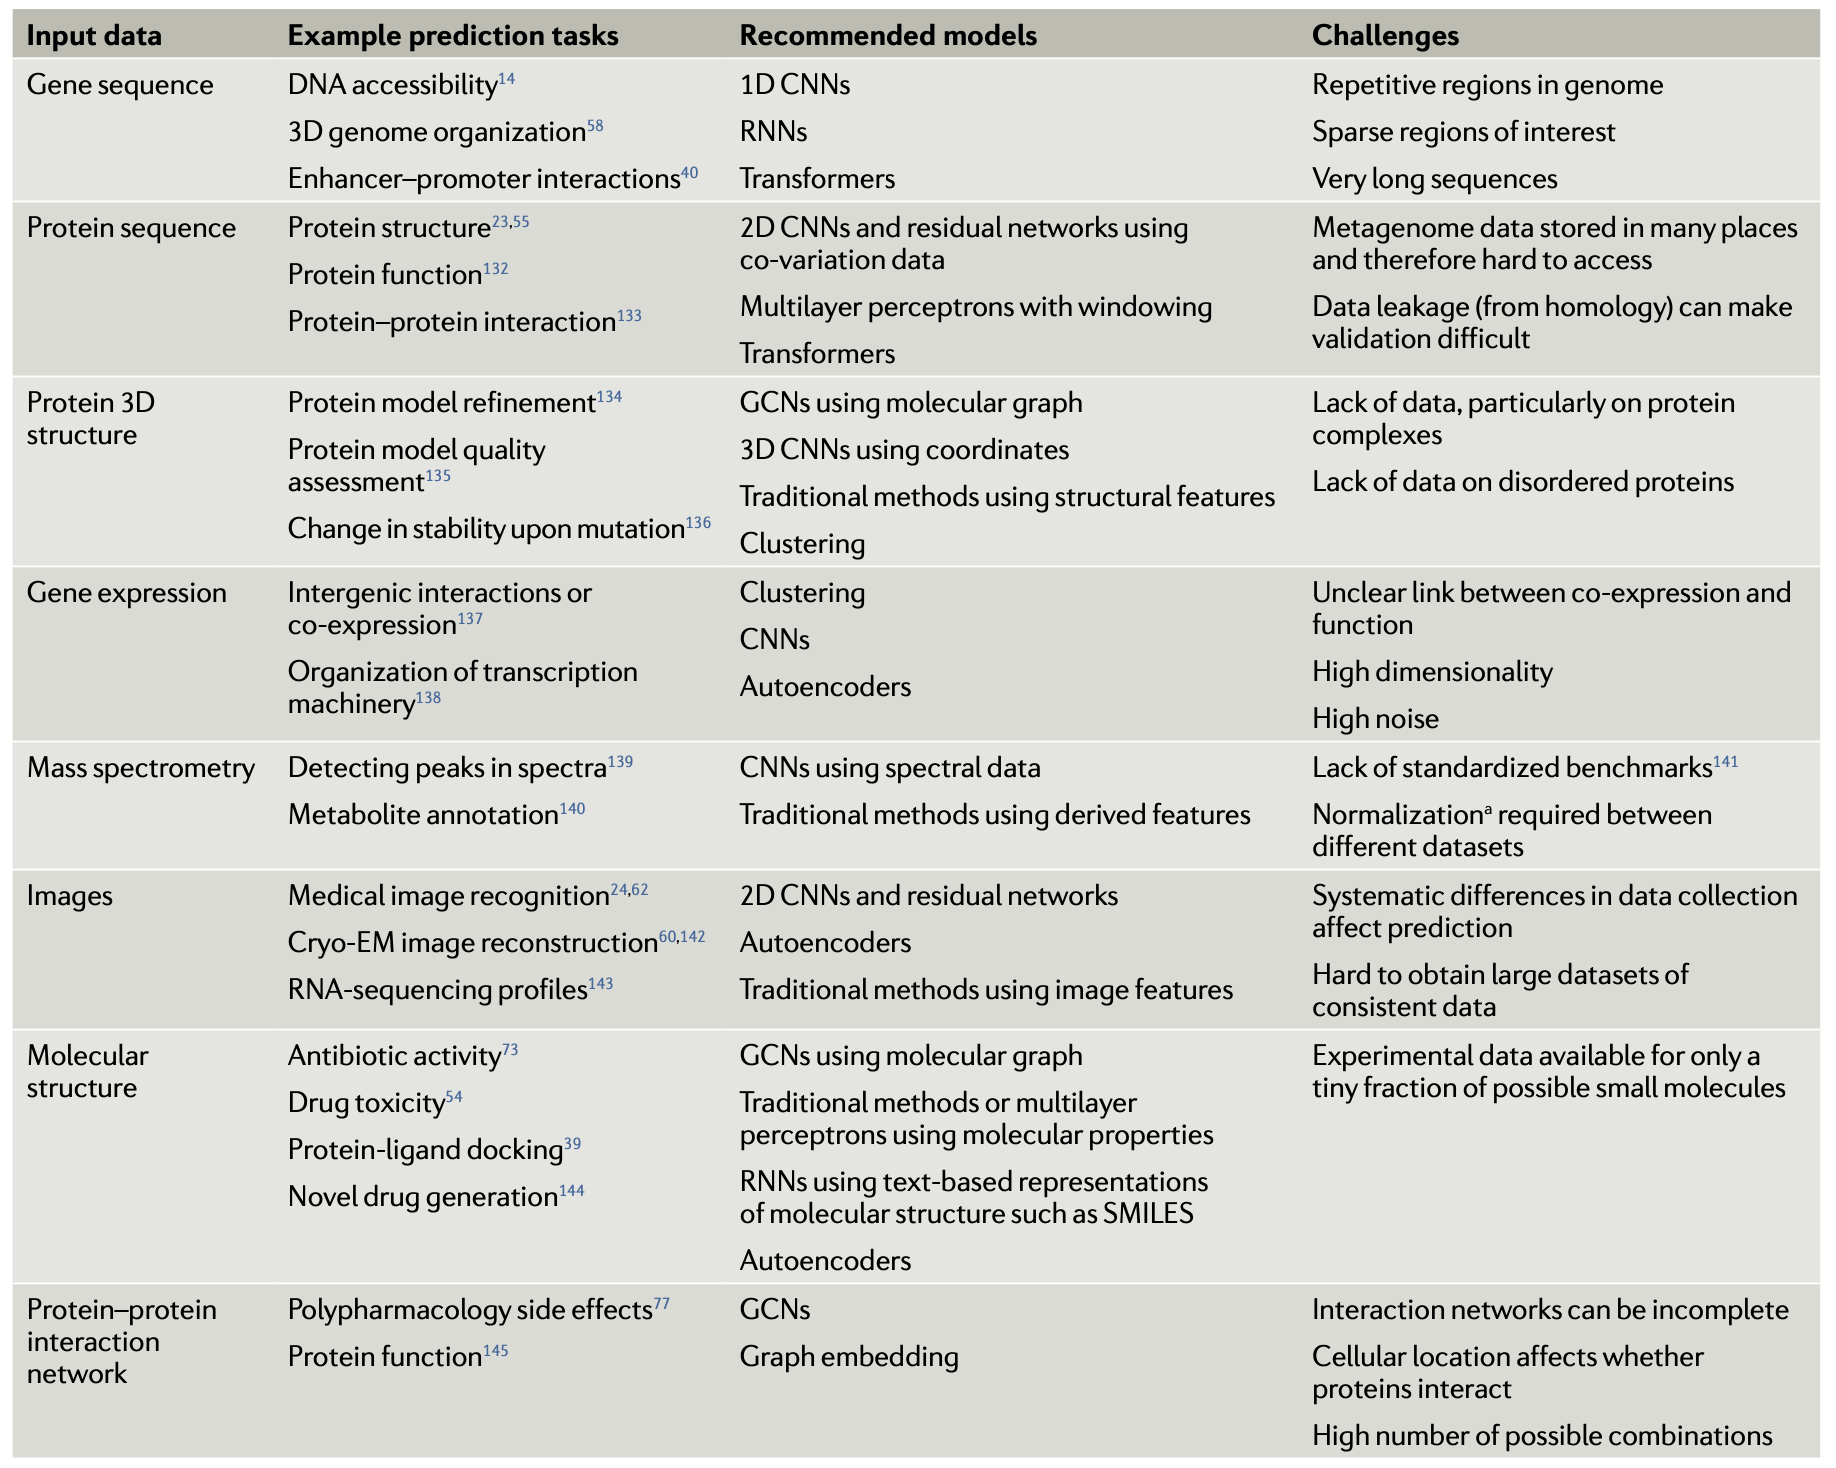
\includegraphics[width = 1\linewidth]{figures/figure_2.png}}
			\caption{Recommendations for the use of machine learning strategies for different biological data types}
		\end{figure}
		
		\section*{Machine Learning in Related Fields}
		
		\subsection*{Distinguishing Venomous Toxins from Other Proteins by Machine Learning\textsuperscript{\cite{ref6}}}
		
		\paragraph*{In this study, a selection of machine learning based classifiers that implement a series of BLAST and HMMER based annotation models were trained on datasets of known toxins, protein sequences that are assumed to be non-toxic but have homology to known toxins, and predicted coding proteins. Present in the genomes, transcriptomes or proteomes of a range of toxic and non-toxic animals. The results show that most machine learning methods consistently outperform standard bioinformatics methods for functional annotation. Interestingly, all tested methods showed higher performance in negative prediction (classification of nontoxic sequences) compared to positive classification (prediction of toxic sequences as toxins). These results suggest that distinguishing physiological toxin-like proteins from actual toxins is more difficult than predicting random proteins to be non-toxic, which is expected given the similarity and common origin of many toxins and toxin-like sequences.}
		
		\paragraph*{This study establishes baseline prediction accuracies for a range of toxin annotation methods and integrates these methods into an easy-to-use, high-precision, machine-learning-based classification system named "ToxClassifier." This tool provides a reliable and reproducible framework for toxin annotation, standardizes toxin prediction in toxicomics projects, and allows semi-automatic annotation or re-annotation of existing datasets.}
		
		\subsection*{Identification of Novel Antimicrobial Peptides in Spider Venom Glands via Deep Learning\textsuperscript{\cite{ref7}}}
		
		\paragraph*{Antimicrobial peptides (AMPs) have recently received a great deal of attention as potential novel therapeutic agents because of their ability to effectively kill a wide range of microorganisms by penetrating biofilms, disrupting cellular components, and inhibiting metabolic processes. In this study, venom gland transcriptomic data were obtained from the spider P. astrigera to identify novel AMPs. Many studies have been based on homology searches when processing transcriptomic data to investigate and characterize animal venoms. However, since homology search is based on sequence similarity to discovered peptides, it has limitations in identifying novel functional peptides that have no sequence similarity to known peptides. In contrast, deep learning methods predict antimicrobial function based on the peptide sequence itself, i.e., antimicrobial activity is predicted based on the sequence of the input amino acids (AAs), without taking into account any physicochemical properties and using only potential representations.}
		
		\paragraph*{In this study, PA-Full and PA-Win were selected from the prediction results using full and partial sequences as input data, respectively.Both peptides were experimentally evaluated and identified as AMPs, and in particular, PA-Win showed excellent antimicrobial activity with low toxicity to mammalian cells. The deep learning model identified novel AMPs that could not be suggested by traditional methods including but not limited to BLAST.Finally, PA-Win showed significant antimicrobial activity comparable to a representative AMP (bee venom peptide) against all tested strains and demonstrated cytocompatibility without hemolytic activity, further enhancing its value. It is demonstrated that by using this development model, it is possible to perform a high-throughput prediction of novel functional peptides at low cost and with little effort, and to mine peptides with high potential and applicability as AMPs, such as PA-Win.}
		
		\subsection*{Prediction of Novel Spider Neurotoxic Peptides by Deep Learning Methods\textsuperscript{\cite{ref8}}}
		
		\paragraph*{As major components of spider venom, neurotoxic peptides exhibit structural diversity, target specificity, and great drug potential. Deep learning may be an alternative to laborious and time-consuming methods for recognizing these peptides. However, a major obstacle to developing deep learning models is the limited data on neurotoxic peptides. This study proposes a peptide data enhancement method to improve the recognition of neurotoxic peptides through convolutional neural network (CNN) models. This peptide data enhancement method enhances the performance of deep learning models for neurotoxicity prediction. The enhancement is performed by generating peptide sequences based on neurotoxic peptides and selecting sequences homologous to known neurotoxic peptides. When the models were trained to use either augmented (AUG) or unaugmented (unAUG) datasets, the models trained with AUG data outperformed the models trained with unAUG data, indicating that the augmentation method fully mimicked the neurotoxicity features.}
		
		\paragraph*{The enhancement method in this study successfully mimicked the characteristics of neurotoxic peptides. The augmented data improved the predictive performance of the deep learning model, which led to the discovery of new peptides. The AUG CNN model predicted putative neurotoxic peptides in the Korean C. koreanus transcriptome, and four selected sequences showed neuromodulatory efficacy. Since the enhancement method is based only on peptide sequences, it can be applied without restriction to develop other predictive models using peptide data. The results suggest that enhancement strategies to improve the identification of novel neurotoxic peptides can broaden the opportunities to study functional bioactive compounds.}
		
		\section*{Conclusion}
		
		\paragraph*{There have been more and more cases where machine learning and especially deep learning methods have been applied to the study of venoms of other species (e.g., spiders). This is because the invocation of deep learning can minimize labor and time costs compared to traditional research protocols, and also has the opportunity to achieve a higher degree of precision in the study of certain problems. Although there may not be much research on ant venom peptides compared to other species, the available research proves that ant venom is similar to the venom of other arthropods. Therefore, it is not difficult to conclude that the use of deep learning has the potential to help evaluate and decipher new molecules of venom peptides from ants. Still, the exact deep learning approach that should be chosen needs to be selected based on the type of data available and guided by the established research objectives.}
		
		\newpage
		
		\begin{thebibliography}{99}  
			\bibitem{ref1}\texttt{Touchard, A., Koh, J. M. S., Aili, S. R., Dejean, A., Nicholson, G. M., Orivel, J. and Escoubas, P. (2015), The complexity and structural diversity of ant venom peptidomes is revealed by mass spectrometry profiling, Rapid Commun. Mass Spectrom., 29, pages 385–396, doi: 10.1002/rcm.7116.}
			
			\bibitem{ref2}\texttt{Samira R. Aili, Axel Touchard, Pierre Escoubas, Matthew P. Padula, Jérôme Orivel, Alain Dejean, Graham M. Nicholson, Diversity of peptide toxins from stinging ant venoms, Toxicon, Volume 92, 2014, Pages 166-178, ISSN 0041-0101, https://doi.org/10.1016/j.toxicon.2014.10.021.}
			
			\bibitem{ref3}\texttt{Touchard A, Téné N, Song PCT, Lefranc B, Leprince J, Treilhou M, Bonnafé E. Deciphering the Molecular Diversity of an Ant Venom Peptidome through a Venomics Approach. J Proteome Res. 2018 Oct 5;17(10):3503-3516. doi: 10.1021/acs.jproteome.8b00452. Epub 2018 Sep 10. PMID: 30149710.}
			
			\bibitem{ref4}\texttt{Wu JP, Li MH. The use of freshwater planarians in environmental toxicology studies: Advantages and potential. Ecotoxicol Environ Saf. 2018 Oct;161:45-56. doi: 10.1016/j.ecoenv.2018.05.057. Epub 2018 May 30. PMID: 29859407.}
			
			\bibitem{ref5}\texttt{Greener, J.G., Kandathil, S.M., Moffat, L. et al. A guide to machine learning for biologists. Nat Rev Mol Cell Biol 23, 40–55 (2022). https://doi.org/10.1038/s41580-021-00407-0}
			
			\bibitem{ref6}\texttt{Gacesa R, Barlow DJ, Long PF. 2016. Machine learning can differentiate venom toxins from other proteins having non-toxic physiological functions. PeerJ Computer Science 2:e90 https://doi.org/10.7717/peerj-cs.90}
			
			\bibitem{ref7}\texttt{Lee B, Shin MK, Yoo JS, Jang W, Sung JS. Identifying novel antimicrobial peptides from venom gland of spider Pardosa astrigera by deep multi-task learning. Front Microbiol. 2022 Aug 24;13:971503. doi: 10.3389/fmicb.2022.971503. PMID: 36090084; PMCID: PMC9449525.}
			
			\bibitem{ref8}\texttt{Lee B, Shin MK, Hwang I-W, Jung J, Shim YJ, Kim GW, Kim ST, Jang W, Sung J-S. A Deep Learning Approach with Data Augmentation to Predict Novel Spider Neurotoxic Peptides. International Journal of Molecular Sciences. 2021; 22(22):12291. https://doi.org/10.3390/ijms222212291}
		\end{thebibliography}
		
	\end{document}